%!TEX root = ../dissertation_vkslm.tex

\chapter{Evaluation Setup}\label{ch:exp}

The quality evaluation of the synthetic signatures has been performed according to the protocol presented by Diaz-Cabrera et al. \cite{diaz2014generation}. A state-of-the-art offline verification system and a dataset including both online and real offline signatures was considered in order to train the system. The main idea of experiments is to measure the quality of the synthetic signatures in terms of performance comparison to the use of only real offline signatures and in inspecting performance variations by increasing the number of training samples with synthetic generated ones.

The goal of the experiments is to measure the quality of the synthetic signatures taking into account an offline verification system performance. The questions raised are \begin{inlinelist}
  \item is the synthetic signatures system performance similar to the offered by real offline signatures?
  \item is it feasible to increase the number of samples at the enrollment stage with our proposed method synthetic signatures? 
\end{inlinelist}



\section{Offline Signature Verification System}
The system used for the evaluation of the real and synthetic signatures is a Linear SVM classifier and with a state-of-the-art feature extraction approach  \cite{hafemann2017learning}. The feature extraction system \footnote{https://www.etsmtl.ca/Unites-de-recherche/LIVIA/Recherche-et-innovation/Projets/Signature-Verification} uses ideas from transfer learning and multi-task learning to learn features using Convolutional Neural Networks (CNN). As discussed in Chapter \ref{ch:nndl}, one of the advantages of using deep learning techniques is that some models, such as the CNN, can learn filters that can be used as feature extractors. The offline system's feature extractor takes advantage of this concept.

\subsection {Support Vector Machine} 
SVMs represent a special class of linear classifiers. In order to classify a pattern as
belonging to one of two classes, an SVM constructs a plane such that it maximally separates the margin between the two classes, as it can be seen in Figure \ref{fig:svm}. For this reason, SVMs are also referred to as maximum margin classifiers.


\begin{figure*}[!htb]
\centering
 \subfloat[The data can be separated using different. lines]{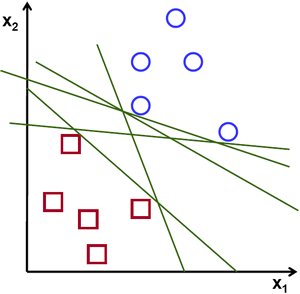
\includegraphics[width=2.3in]{separating-lines}} 
\hspace*{0.5in} % separation between the subfigures
\subfloat[The SVM strives for the optimal line, which maximally separates the margin between the two classes of data.] {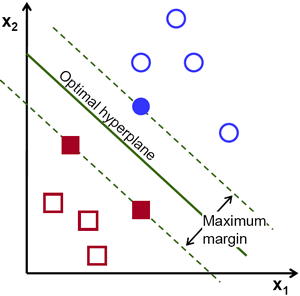
\includegraphics[width=2.3in]{optimal-hyperplane}}

\caption{Illustration of several separating lines and an optimal line.} \label{fig:svm}
\end{figure*}


\section{Evaluation Database}

The evaluation experiments were carried out on the BiosecurID database \cite{biosecurid}. This multimodal database was made publicly available containing signatures of 132 subjects. Signatures were captured using a special digital inking pen on a paper placed over a digitizing tablet, exactly as shown in Figure \ref{fig:onoff}. Consequently, both versions, online and offline, of the same real signature were acquired at the same time. This characteristic, therefore, makes BiosecurID the ideal benchmark for the experimental evaluation conducted in this work.


The signatures samples were captured in 4 different sessions, distributed over four months. Each subject signed 4 times and forged 3 signatures per session, thus leading to each subject having 4 genuine signatures x 4 sessions = 16 genuine samples and 3 signature forgeries x 4 sessions = 12 skilled forgeries.

Since the offline signature verification system is trained with both positive and negative samples, to ensure an unbiased result towards the dataset selection, similar to the protocol followed by \cite{diaz2014generation} we used the MCYT database \cite{mcyt-100} as the negative dataset samples. The MCYT dataset includes 75 signers each with 15 genuine and 15 skilled forged signatures. The amount of negative samples was set to 25 random samples from the MCYT dataset.



\section{Experimental Protocol}
In order to accomplish a fair comparison of our work and the state of the art, the same experiment protocol proposed by \cite{diaz2014generation} has been adopted. More specifically, two different experiments are carried out: Experiment 1 focuses on evaluating the synthetic signatures performance in comparison to real signatures; Experiment 2 evaluates the feasibility of synthetically increasing the number of samples available in a dataset.

For both experiments the BiosecurID dataset is split into two subsets. According to \cite{diaz2014generation}, the first 90 users are used as the enrollment set in order to compute the genuine and skilled impostor scores. The remaining 42 users are considered as the test set and are used to compute the random impostor scores. The performance is evaluated in terms of equal error rate (EER), which is the point in the Detection Error Tradeoff curve (DET) where the false acceptance rate equals the false rejection rate. We report the details of experiments setup for an easy reading of the paper.

\begin{itemize}
	\item Experiment 1:Two different protocols in order to train the system are considered:	
	\begin{inlinelist}
		\item mono-session: four samples of the first acquisition session are used;
		\item multi-session: one sample of each of the 4 acquisition sessions are used
	\end{inlinelist}. Genuine scores are evaluated using the user’s genuine samples not used in enrollment. Random forgery scores are evaluated by comparing the first sample of the test subjects to the enrolled model. Skilled forgery scores are evaluated with the skilled forgeries samples of the enrolled users.
	
	\item Experiment 2: This experiment is designed to assess whether synthetically increasing the enrollment dataset leads to a better recognition performance. The evaluation is made through three different enrollment sets:
	\begin{itemize}
		\item 4 real samples from the first acquisition session
		\item 4 real samples from the first plus 4 real samples from the second session
		\item 4 real samples from the first session plus 4 synthetic samples of the second session.
	\end{itemize}
	
\end{itemize}

\begin{figure}[!htb]
	\centering
	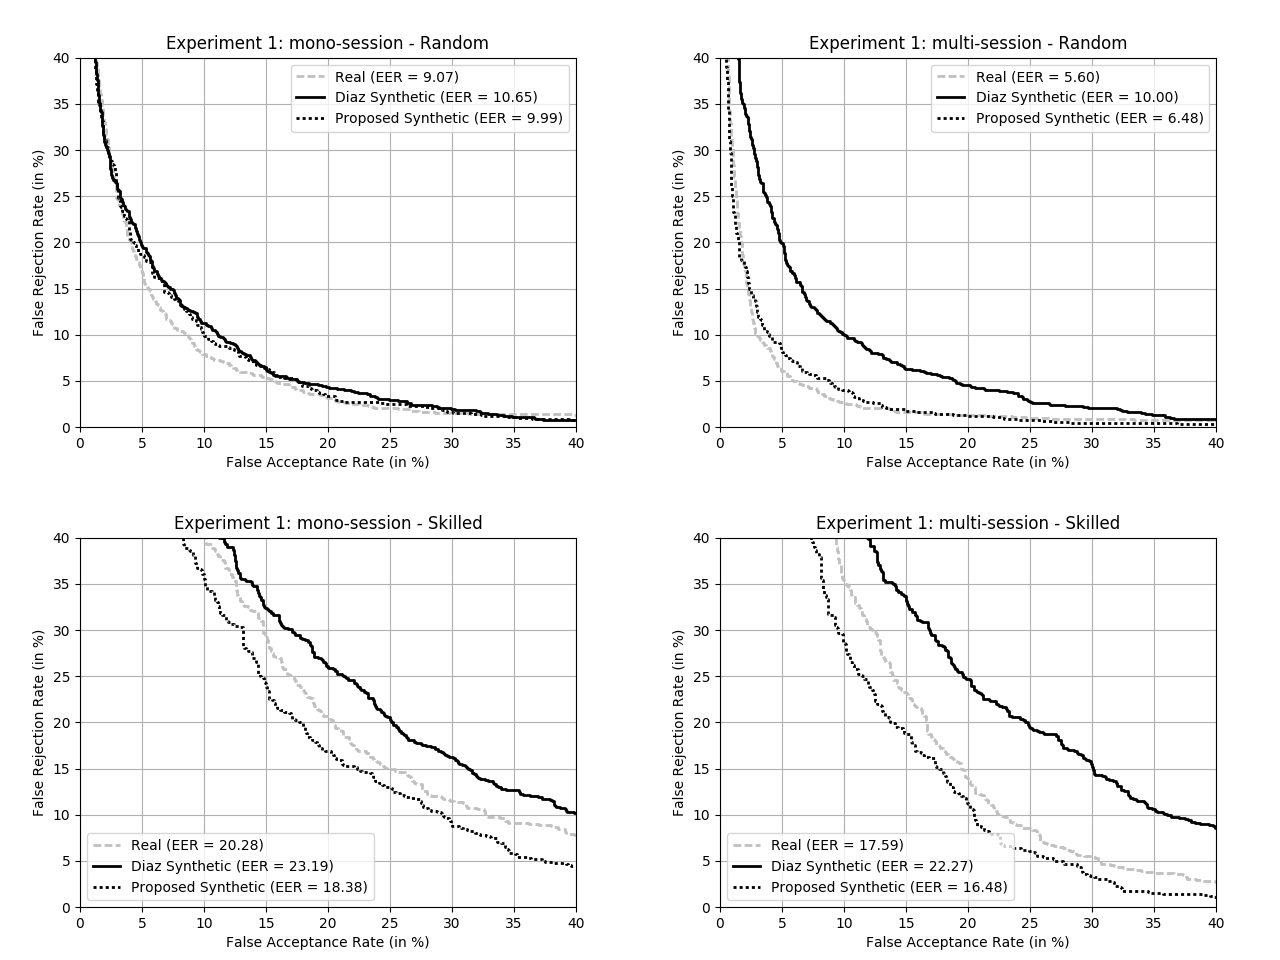
\includegraphics[width=5.4in]{rocs/experiment1}
	% where an .eps filename suffix will be assumed under latex,
	% and a .pdf suffix will be assumed for pdflatex; or what has been declared
	% via \DeclareGraphicsExtensions.
	\caption{DET curves for real offline signatures and synthetic signatures (from Diaz and our proposed method), for the first experiment (mono-session and multi-session enrollment), for the two scenarios considered (random and skilled impostors)}
	\label{exp1}
\end{figure}



\section{Performance Assessment}

AHSVS efficiency is quantitatively measured by two rates: False Rejection Rate (FRR) which is the percentage of genuine signatures treated as forgeries, and False
Acceptance Rate (FAR) which is the percentage of forged signatures treated as
genuine. 

A derived metric usually reported is the Average Error rate (AER) which is the average of FAR and FRR. Moreover, when experimenting an AHSVS, the trade-off between FRR and FAR must be taken into account based on the type of application and other aspects related to where the system is used. When the decision threshold of a system is set to have the FRR approximately equal to the FAR, the Equal Error Rate (EER) is calculated. In our experimental results, the system's EER performance is reported.

%Besides quantitative results, the performance can be also compared and visualized using graphs. Receiver operating characteristics (ROC) graphs have been used increasingly in machine learning and data mining research \cite{fawcett2006introduction}. Inicialmente, a curva ROC foi desenvolvida para demonstrar as relações sinal-ruído,
%interpretando o sinal como verdadeiros positivos (sensibilidade) e o ruído, os falsos positivos
%(especificidade). Assim, a leitura da curva ROC é de um gráfico de sensibilidade ou taxas de
%verdadeiros positivos versus taxa de falsos positivos, como apresentado na Figura 26. Os
%gráficos ROC são bidimensionais, estando o eixo Y com os valores verdadeiros positivos e o
%eixo X preenchido com os valores da taxa falsos positivo.
%
%O objetivo da ferramenta curva ROC é atingir a representação perfeita do experimento,
%considerando o conjunto de amostras analisado.
%O objeto de estudo tem sua avaliaçãoidentificada pela localidade do ponto no gráfico. Quão mais próximo o ponto estiver do eixo Y,
%melhor será o resultado. Assim, a diagonal traçada do ponto (0,0) ao ponto (1,1) serve de
%direcionamento para identificar quais são os melhores resultados, estes localizados
%predominantemente acima da reta [FAWCELT, 2006]. 
%
%A métrica utilizada no estudo do ICDAR 2009 [BLANKERS et al, 2009] foi a Detection
%Error Trade-off curve (DET) [MARTIN, 1997] (gráfico visualizado na Figura 28). Esta métrica
%é mais conhecida como a curva DET. Esta curva corresponde a um gráfico que estabelece uma
%relação entre as taxas de erro diferentemente da curva ROC. A curva é definida como a linha
%contendo os pontos onde x = y, ou seja, posição onde os erros FRR e FAR possuem o mesmo
%valor. Assim, o gráfico é gerado baseando-se na taxa EER. No gráfico DET o melhor resultado
%está localizado o mais próximo do eixo inicial (o ponto 0 (zero)). O mais próximo apresenta,
%assim, o menor erro de classificação. Esta métrica foi utilizada pelo ICDAR para definir o
%algoritmo de classificação da competição com o melhor EER nos problemas de verificação de
%assinaturas nos modos off-line e on-line.

%\section{Statistical Evaluation}


